\documentclass{article}
 
\usepackage{color}
\usepackage{listings}
\usepackage{graphicx}
\usepackage{subfig}

\definecolor{MyYellow}{rgb}{1,1,0.8}
 
\lstset{language=Matlab,backgroundcolor=\color{MyYellow},basicstyle=\footnotesize,numberstyle=\footnotesize,numbers=left,stepnumber=1,numbersep=5pt,breaklines=true,frame=lines,tabsize=2}
 
\author{Ruurd Moelker \and Jan Paul Posma}
\date{\today}
\title{Signalen \& Systemen \\Practicum 3}

\begin{document}
\maketitle
 
\section{Opgave 1}
Om de convolutie in matlab te bepalen gebruiken wij het commando:
$conv(xx,~[1,~-0.9])$
De filterco\"efici\"enten zijn hierbij 1 en 0.9.

Het invoersignaal $x[n]$ is de reeks van getallen startende met 10 maal 256 gevolgd door 40 maal een 0 waarna de reeks zich herhaald tot 100 getallen zijn bereikt.

\section{Opgave 2}
De stemplot van x[n] in te zien samen met de stemplot van w[n] in figuur \ref{fig:opgave2}.

\begin{figure}[h]
  \centering
 	\subfloat[][x[n]]{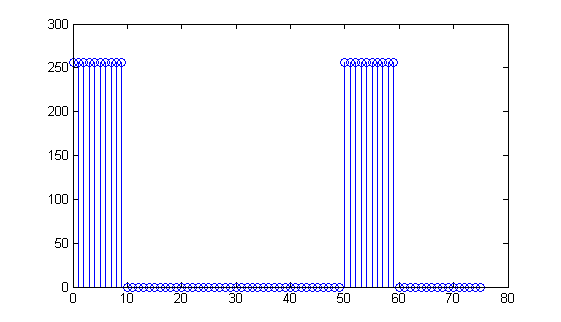
\includegraphics[width=0.4\textwidth]{content/2xx.png}}
	\subfloat[][w[n]]{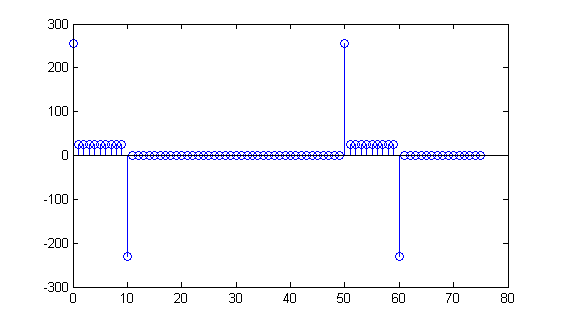
\includegraphics[width=0.4\textwidth]{content/2ww.png}}
  \caption{Stemplot van x en w over het interval [0..75]}
  \label{fig:opgave2}
\end{figure}

\section{Opgave 3}
Het matlab commando $length()$ geeft de lengte van een signaal. Voor x[n] is deze lengte 101 en voor w[n] is de lengte 102. De lengte van de convolutie wordt inderdaad bepaald door $length(xx)+length(bb)-1$ waarbij bb de vector met co\"efficienten is, in dit geval [1, -0.9], dus lengte 2.

\section{Opgave 4}
$r = 0.9$
$M = 22$
$rr = r .^ (0:M)$
$yy = conv(ww, rr)$

\section{Opgave 5}
In figuur \ref{fig:opgave5} is de benadering van $x[n]$ door de convolutie van de reeks $rr$ op $w[n]$ geplot in een stem grafiek.
\begin{figure}[h]
  \centering
 	\subfloat[][w]{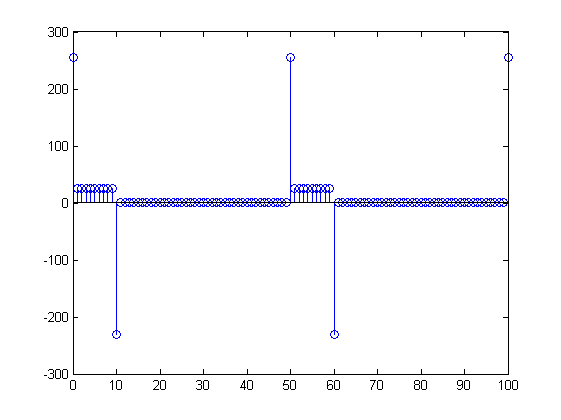
\includegraphics[width=0.4\textwidth]{content/5ww.png}}
	\subfloat[][y]{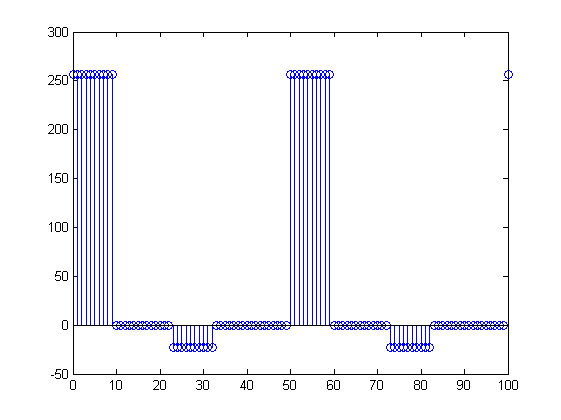
\includegraphics[width=0.4\textwidth]{content/5yy.png}}
  \caption{Stemplot van w en de benadering van w van x}
  \label{fig:opgave5}
\end{figure}
\section{Opgave 6}
In figuur \ref{fig:opgave6}
\begin{figure}[h]
  \centering
 	\subfloat[][x]{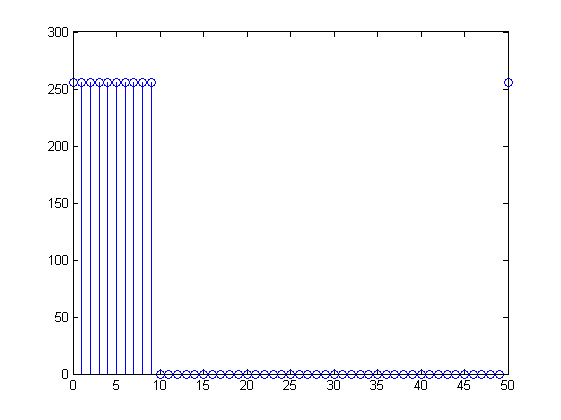
\includegraphics[width=0.4\textwidth]{content/6xx.png}}
	\subfloat[][y]{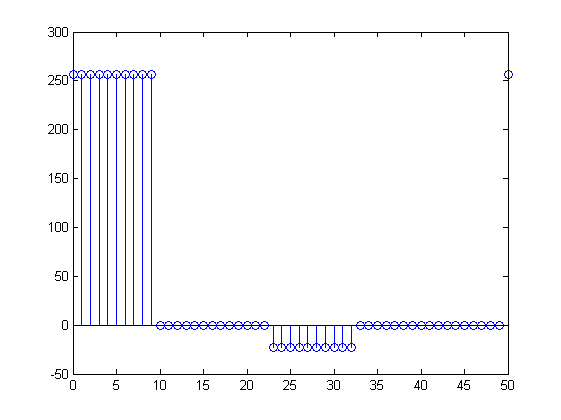
\includegraphics[width=0.4\textwidth]{content/6yy.png}}
	\subfloat[][x-y]{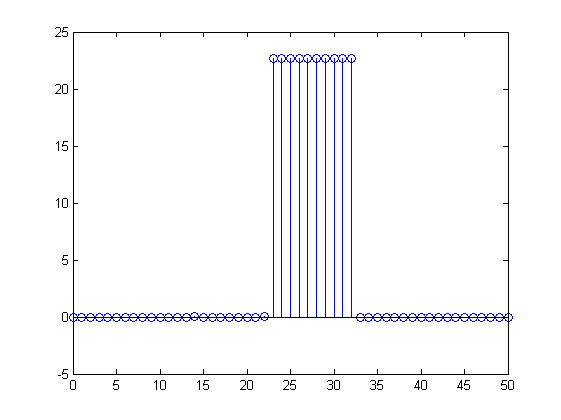
\includegraphics[width=0.4\textwidth]{content/6.png}}
  \caption{!!!!!!!!!}
  \label{fig:opgave6}
\end{figure}

\section{Opgave 7}
De waarde van r wordt bepaald door de sterkte die we aan de echo toekennen, het is immers de amplitude van het signaal P tijdeenheden terug dus: $r = 0.9$. P is de tijdverschuiving van de echo uigedrukt in tijdseenheden van de sample frequentie dus $p = \delta~t*f_s = 8000 * 0.2 = 1600$.

\section{Opgave 8}
De echo van een signaal kan met een FIR filter met convolutie $[1, 0_1 .. 0_p-1, 0.9]$ gemaakt worden. In matlab wordt het nieuwe signaal yy uit bronsignaal x2 berekend: $yy = conv(x2, [1 zeros(1,8000*0.2 - 1) 0.9]);$. Het oorspronkelijke signaal x2 en gefilterd signaal yy zijn uitgezet in figuur \ref{fig:opgave8}.
\begin{figure}[h]
  \centering
 	\subfloat[][x2]{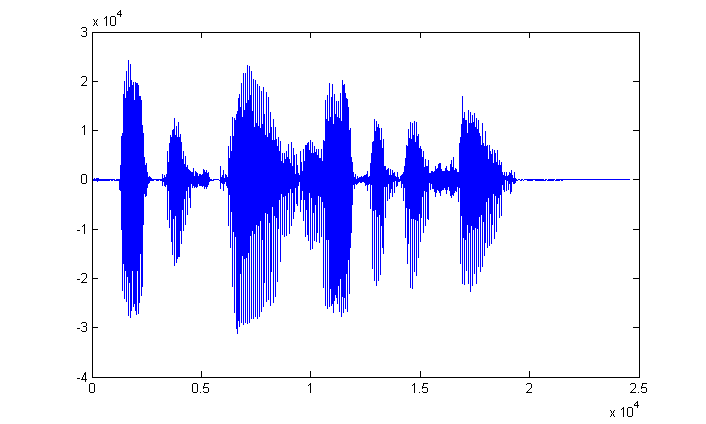
\includegraphics[width=0.4\textwidth]{content/8x2.png}}
	\subfloat[][yy]{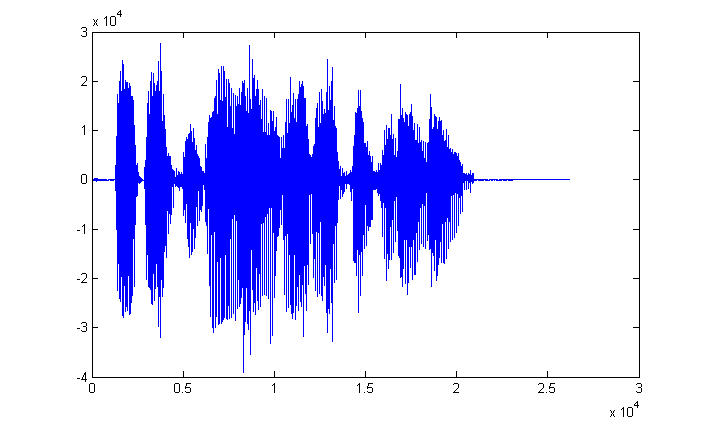
\includegraphics[width=0.4\textwidth]{content/8yy.png}}
  \caption{Het orginele signaal x2 verkregen uit functie labdat.mat en het signaal met echo yy}
  \label{fig:opgave8}
\end{figure}

\end{document}